% Section content template for individual Educative lessons
% This file contains the actual content for a specific section
% Generated from Educative API section content

% Section: Use Case Diagram for the ATM System
% Section ID: 5191075351494656
% Section Slug: use-case-diagram-for-the-atm-system
% Generated: 2025-12-12T15:53:13.003327

Let's build the ATM system's use case diagram and understand the relationship between its main actors and functions. First , we'll define the different elements of our system, followed by the complete use case diagram.

\subsection{System}\label{QoayzELP223HIjx5bzBv0}
\\
Our system is the ATM system. It manages secure, card-based access for bank customers to perform key banking transactions remotely.

\subsection{Actors}\label{hK2hPJCBRNicC5p8f6lGE}
\\
Let's define the main actors of our ATM system.

\subsubsection{Primary actor}\label{UVp-MTI1W-7duvN17j3JK}

\begin{itemize}
\item
\protect\phantomsection\label{sGlY9A4guN3p8gOc7papt}
\textbf{Cardholder:} The user who interacts with the ATM to perform banking transactions such as inserting/removing the card, entering PIN, and carrying out account operations.
\end{itemize}

\subsection{Use cases}\label{lKpx0WM5oT39Q2zkErepi}
\\
In this section, we will define the ATM's use cases. We have listed them according to their interactions with a particular actor.

\subsubsection{Cardholder}\label{GYH3_q-nOn9lmEi-o1RJs}

\begin{itemize}
\item
\textbf{Insert card:} To insert the ATM card into the machine.
\item
\textbf{Enter PIN:} To enter their PIN to verify identity.
\item
\textbf{Change PIN:} To change the card's PIN.
\item
\textbf{Select transaction:} To initiate a transaction (generalization of the next four):

\begin{itemize}
\item
\textbf{Balance inquiry:} To check the account balance.
\item
\textbf{Funds transfer:} To transfer money between accounts.
\item
\textbf{Cash withdrawal:} To withdraw the cash.
\end{itemize}
\item
\textbf{Enter amount:} To enter the amount they want to transfer or withdraw.
\item
\textbf{Cancel transaction:} To cancel a transaction.
\end{itemize}

\subsubsection{ATM system}\label{vrrcj-1XBKwB3M635KTmS}

\begin{itemize}
\item
\textbf{Verify cardholder identity:} To validate the card and the cardholder's credentials.
\item
\textbf{Check withdrawal limits:} To validate the ATM's transaction limits and the cardholder's bank limits.
\item
\textbf{Check account transaction limits:} To validate that the transaction is within the account's permissible limits.
\item
\textbf{Return card:} To eject the card after the transaction or cancellation.
\item
\textbf{Dispense money:} To dispense cash during withdrawal.
\item
\textbf{Diispense receipt:} To print and provide a receipt for the transaction.
\end{itemize}

\subsection{Relationships}\label{sNsTucwzYvKTF86L2rNsn}
\\
This section describes the relationships between and among actors and their use cases.

\subsubsection{Associations}\label{DwYk6UWJaCZK-xTeM8qpA}
\\
The table below shows the association relationship between actors and their use cases.

\begin{center}
{\def\LTcaptype{none} % do not increment counter
\begin{longtable}[]{@{}
>{\raggedright\arraybackslash} p{(\linewidth - 2\tabcolsep) * \real{0.5000}}
>{\raggedright\arraybackslash} p{(\linewidth - 2\tabcolsep) * \real{0.5000}}@{}}
\toprule\noalign{}
\endhead
\bottomrule\noalign{}
\endlastfoot
\begin{minipage}[t]{\linewidth}\raggedright
\textbf{Cardholder}
\end{minipage} & \begin{minipage}[t]{\linewidth}\raggedright
\textbf{ATM System}
\end{minipage} \\
\begin{minipage}[t]{\linewidth}\raggedright
Insert card
\end{minipage} & \begin{minipage}[t]{\linewidth}\raggedright
Verify cardholder identity
\end{minipage} \\
\begin{minipage}[t]{\linewidth}\raggedright
Enter PIN
\end{minipage} & \begin{minipage}[t]{\linewidth}\raggedright
Check withdrawal limits
\end{minipage} \\
\begin{minipage}[t]{\linewidth}\raggedright
Change PIN
\end{minipage} & \begin{minipage}[t]{\linewidth}\raggedright
Check account transaction limits
\end{minipage} \\
\begin{minipage}[t]{\linewidth}\raggedright
Select transaction
\end{minipage} & \begin{minipage}[t]{\linewidth}\raggedright
Return card
\end{minipage} \\
\begin{minipage}[t]{\linewidth}\raggedright
Enter amount
\end{minipage} & \begin{minipage}[t]{\linewidth}\raggedright
Dispense money
\end{minipage} \\
\begin{minipage}[t]{\linewidth}\raggedright
Cancel transaction
\end{minipage} & \begin{minipage}[t]{\linewidth}\raggedright
Dispense receipt
\end{minipage} \\
\end{longtable}
}
\end{center}

\subsubsection{Include}\label{guYaczFFXYfD3wD7jLEZB}
\\
When cardholders initiate an ATM session, they must verify their identity by entering their PIN. This process is enforced using ``include'' relationships in the use case diagram:

\begin{itemize}
\item
\protect\phantomsection\label{0gRKiNPrT-95pBtAqSBaf}
The ``Insert card'' use case includes the ``Enter PIN'' use case.
\item
\protect\phantomsection\label{vx5pM9WS7bZXuLIN0wYVE}
The ``Enter PIN'' use case includes the ``Verify cardholder identity'' use case.
\end{itemize}
\\
Before a cardholder can change their PIN, the system must authenticate them:

\begin{itemize}
\item
\protect\phantomsection\label{K1N2JSv8iC4i1o8fVHzry}
The ``Change PIN'' use case includes the ``Enter PIN'' use case and then the ``Verify cardholder identity'' use case.
\end{itemize}
\\
When a cardholder chooses to perform a transaction, they must select from the available transaction types:

\begin{itemize}
\item
\protect\phantomsection\label{qyG1vmcyMKGnKxIW4Gv-N}
The ``Select transaction'' use case includes the ``Balance inquiry'', ``Funds transfer'', and ``Cash withdrawal'' use cases.
\end{itemize}
\\
For ``Funds transfer'' and ``Cash withdrawal'', the cardholder must specify the amount to transfer or withdraw:

\begin{itemize}
\item
\protect\phantomsection\label{EhSYwWF6h8Bbw8hXUKlX-}
The ``Funds transfer'' and ``Cash withdrawal'' use cases include the ``Enter amount'' use case.
\end{itemize}
\\
When the cardholder enters an amount to withdraw, the system must ensure all limits are respected:

\begin{itemize}
\item
\protect\phantomsection\label{rZjq-Gz9JifK3PLDMVNKV}
The ``Enter amount'' use case includes the ``Check withdrawal limits'' use case.
\item
\protect\phantomsection\label{abgozPOhDMbkgvm2uumlA}
The ``Check withdrawal limits'' use case includes the ``Check account transaction limits'' use case.
\end{itemize}
\\
After a transaction (such as a balance inquiry, funds transfer, or cash withdrawal), the system provides a receipt to the cardholder if requested:

\begin{itemize}
\item
\protect\phantomsection\label{djH6C03svGp39uYdcljE2}
The ``Balance inquiry'' and ``Cash withdrawal'' use cases each include the ``Dispense receipt'' use case.
\end{itemize}
\\
If the cardholder cancels a transaction or ends their session, the ATM must return the card:

\begin{itemize}
\item
\protect\phantomsection\label{w65_67ZH8KM1oHo1DM9W9}
The ``Cancel transaction'' use case includes the ``Return card'' use case.
\item
\protect\phantomsection\label{D_r39aKNdB08zI6FLXrPe}
At the end of any session, the ``Return card'' use case is always included to ensure the cardholder retrieves their card.
\end{itemize}

\subsection{Use case diagram}\label{LYOMcdwdnvyk4vyRs7Yiz}
\\
Here's the use case diagram of the ATM design:

\begin{figure}[htbp]
 \centering
 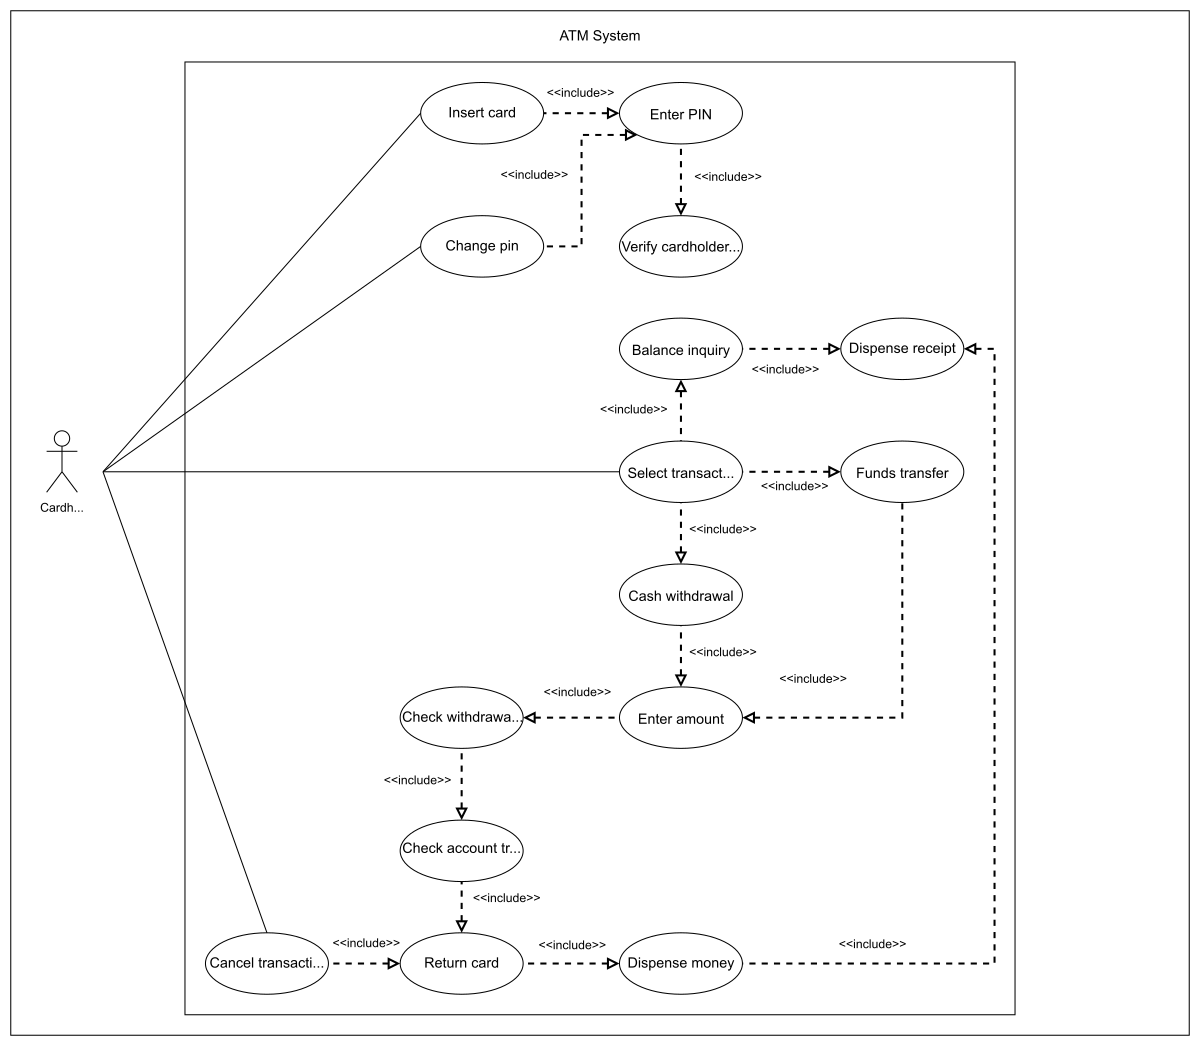
\includegraphics[width=0.5\textwidth]{Images/chapter_16/section_5191075351494656/5644210794266624.png}
 \caption{The use case diagram of the ATM system}
\end{figure}

In the next lesson, we will discuss the class diagram and explain all classes and their relationships.

% End of section content